\documentclass[twoside]{book}

% Packages required by doxygen
\usepackage{calc}
\usepackage{doxygen}
\usepackage{graphicx}
\usepackage[utf8]{inputenc}
\usepackage{makeidx}
\usepackage{multicol}
\usepackage{multirow}
\usepackage{textcomp}
\usepackage[table]{xcolor}

% Font selection
\usepackage[T1]{fontenc}
\usepackage{mathptmx}
\usepackage[scaled=.90]{helvet}
\usepackage{courier}
\usepackage{amssymb}
\usepackage{sectsty}
\renewcommand{\familydefault}{\sfdefault}
\allsectionsfont{%
  \fontseries{bc}\selectfont%
  \color{darkgray}%
}
\renewcommand{\DoxyLabelFont}{%
  \fontseries{bc}\selectfont%
  \color{darkgray}%
}

% Page & text layout
\usepackage{geometry}
\geometry{%
  a4paper,%
  top=2.5cm,%
  bottom=2.5cm,%
  left=2.5cm,%
  right=2.5cm%
}
\tolerance=750
\hfuzz=15pt
\hbadness=750
\setlength{\emergencystretch}{15pt}
\setlength{\parindent}{0cm}
\setlength{\parskip}{0.2cm}
\makeatletter
\renewcommand{\paragraph}{%
  \@startsection{paragraph}{4}{0ex}{-1.0ex}{1.0ex}{%
    \normalfont\normalsize\bfseries\SS@parafont%
  }%
}
\renewcommand{\subparagraph}{%
  \@startsection{subparagraph}{5}{0ex}{-1.0ex}{1.0ex}{%
    \normalfont\normalsize\bfseries\SS@subparafont%
  }%
}
\makeatother

% Headers & footers
\usepackage{fancyhdr}
\pagestyle{fancyplain}
\fancyhead[LE]{\fancyplain{}{\bfseries\thepage}}
\fancyhead[CE]{\fancyplain{}{}}
\fancyhead[RE]{\fancyplain{}{\bfseries\leftmark}}
\fancyhead[LO]{\fancyplain{}{\bfseries\rightmark}}
\fancyhead[CO]{\fancyplain{}{}}
\fancyhead[RO]{\fancyplain{}{\bfseries\thepage}}
\fancyfoot[LE]{\fancyplain{}{}}
\fancyfoot[CE]{\fancyplain{}{}}
\fancyfoot[RE]{\fancyplain{}{\bfseries\scriptsize Generated on Sat Apr 25 2015 10\-:02\-:54 for Calculator by Doxygen }}
\fancyfoot[LO]{\fancyplain{}{\bfseries\scriptsize Generated on Sat Apr 25 2015 10\-:02\-:54 for Calculator by Doxygen }}
\fancyfoot[CO]{\fancyplain{}{}}
\fancyfoot[RO]{\fancyplain{}{}}
\renewcommand{\footrulewidth}{0.4pt}
\renewcommand{\chaptermark}[1]{%
  \markboth{#1}{}%
}
\renewcommand{\sectionmark}[1]{%
  \markright{\thesection\ #1}%
}

% Indices & bibliography
\usepackage{natbib}
\usepackage[titles]{tocloft}
\setcounter{tocdepth}{3}
\setcounter{secnumdepth}{5}
\makeindex

% Hyperlinks (required, but should be loaded last)
\usepackage{ifpdf}
\ifpdf
  \usepackage[pdftex,pagebackref=true]{hyperref}
\else
  \usepackage[ps2pdf,pagebackref=true]{hyperref}
\fi
\hypersetup{%
  colorlinks=true,%
  linkcolor=blue,%
  citecolor=blue,%
  unicode%
}

% Custom commands
\newcommand{\clearemptydoublepage}{%
  \newpage{\pagestyle{empty}\cleardoublepage}%
}


%===== C O N T E N T S =====

\begin{document}

% Titlepage & ToC
\hypersetup{pageanchor=false}
\pagenumbering{roman}
\begin{titlepage}
\vspace*{7cm}
\begin{center}%
{\Large Calculator }\\
\vspace*{1cm}
{\large Generated by Doxygen 1.8.6}\\
\vspace*{0.5cm}
{\small Sat Apr 25 2015 10:02:54}\\
\end{center}
\end{titlepage}
\clearemptydoublepage
\tableofcontents
\clearemptydoublepage
\pagenumbering{arabic}
\hypersetup{pageanchor=true}

%--- Begin generated contents ---
\chapter{I\-V\-S-\/calculator}
\label{md_README}
\hypertarget{md_README}{}
\input{md_README}
\chapter{Hierarchical Index}
\section{Class Hierarchy}
This inheritance list is sorted roughly, but not completely, alphabetically\-:\begin{DoxyCompactList}
\item \contentsline{section}{Evaluator}{\pageref{classEvaluator}}{}
\item exception\begin{DoxyCompactList}
\item \contentsline{section}{Lexical\-Exception}{\pageref{classLexicalException}}{}
\item \contentsline{section}{Math\-Exception}{\pageref{classMathException}}{}
\item \contentsline{section}{Syntax\-Exception}{\pageref{classSyntaxException}}{}
\end{DoxyCompactList}
\item \contentsline{section}{Math}{\pageref{classMath}}{}
\item \contentsline{section}{Parser}{\pageref{classParser}}{}
\item Q\-Main\-Window\begin{DoxyCompactList}
\item \contentsline{section}{Main\-Window}{\pageref{classMainWindow}}{}
\end{DoxyCompactList}
\item Q\-Object\begin{DoxyCompactList}
\item \contentsline{section}{math\-Test\-Header}{\pageref{classmathTestHeader}}{}
\end{DoxyCompactList}
\item \contentsline{section}{Scanner}{\pageref{classScanner}}{}
\item \contentsline{section}{Token}{\pageref{classToken}}{}
\begin{DoxyCompactList}
\item \contentsline{section}{Function\-Token}{\pageref{classFunctionToken}}{}
\item \contentsline{section}{Number\-Token}{\pageref{classNumberToken}}{}
\end{DoxyCompactList}
\item \contentsline{section}{Token\-Vector}{\pageref{classTokenVector}}{}
\end{DoxyCompactList}

\chapter{Class Index}
\section{Class List}
Here are the classes, structs, unions and interfaces with brief descriptions\-:\begin{DoxyCompactList}
\item\contentsline{section}{\hyperlink{classEvaluator}{Evaluator} }{\pageref{classEvaluator}}{}
\item\contentsline{section}{\hyperlink{classFunctionToken}{Function\-Token} }{\pageref{classFunctionToken}}{}
\item\contentsline{section}{\hyperlink{classLexicalException}{Lexical\-Exception} }{\pageref{classLexicalException}}{}
\item\contentsline{section}{\hyperlink{classMainWindow}{Main\-Window} }{\pageref{classMainWindow}}{}
\item\contentsline{section}{\hyperlink{classMath}{Math} }{\pageref{classMath}}{}
\item\contentsline{section}{\hyperlink{classMathException}{Math\-Exception} }{\pageref{classMathException}}{}
\item\contentsline{section}{\hyperlink{classmathTestHeader}{math\-Test\-Header} }{\pageref{classmathTestHeader}}{}
\item\contentsline{section}{\hyperlink{classNumberToken}{Number\-Token} }{\pageref{classNumberToken}}{}
\item\contentsline{section}{\hyperlink{classParser}{Parser} }{\pageref{classParser}}{}
\item\contentsline{section}{\hyperlink{classScanner}{Scanner} }{\pageref{classScanner}}{}
\item\contentsline{section}{\hyperlink{classSyntaxException}{Syntax\-Exception} }{\pageref{classSyntaxException}}{}
\item\contentsline{section}{\hyperlink{classToken}{Token} }{\pageref{classToken}}{}
\item\contentsline{section}{\hyperlink{classTokenVector}{Token\-Vector} }{\pageref{classTokenVector}}{}
\end{DoxyCompactList}

\chapter{File Index}
\section{File List}
Here is a list of all documented files with brief descriptions\-:\begin{DoxyCompactList}
\item\contentsline{section}{inc/core/{\bfseries evaluator.\-h} }{\pageref{evaluator_8h}}{}
\item\contentsline{section}{inc/core/\hyperlink{math_8h}{math.\-h} \\*\hyperlink{classMath}{Math} \hyperlink{math_8cpp}{math.\-cpp} }{\pageref{math_8h}}{}
\item\contentsline{section}{inc/core/\hyperlink{myexception_8h}{myexception.\-h} \\*Myexception myexception.\-cpp }{\pageref{myexception_8h}}{}
\item\contentsline{section}{inc/core/\hyperlink{parser_8h}{parser.\-h} \\*\hyperlink{classParser}{Parser} \hyperlink{parser_8cpp}{parser.\-cpp} }{\pageref{parser_8h}}{}
\item\contentsline{section}{inc/core/\hyperlink{scanner_8h}{scanner.\-h} \\*\hyperlink{classScanner}{Scanner} \hyperlink{scanner_8cpp}{scanner.\-cpp} }{\pageref{scanner_8h}}{}
\item\contentsline{section}{inc/core/\hyperlink{token_8h}{token.\-h} \\*\hyperlink{classToken}{Token} \hyperlink{token_8cpp}{token.\-cpp} }{\pageref{token_8h}}{}
\item\contentsline{section}{inc/gui/\hyperlink{mainwindow_8h}{mainwindow.\-h} \\*Mainwindow mainwindow.\-cpp }{\pageref{mainwindow_8h}}{}
\item\contentsline{section}{inc/tests/\hyperlink{mathTestHeader_8h}{math\-Test\-Header.\-h} \\*Math\-Test\-Header math\-Test\-Header.\-cpp }{\pageref{mathTestHeader_8h}}{}
\item\contentsline{section}{src/core/\hyperlink{math_8cpp}{math.\-cpp} \\*Mathematical library including primary operations and functions }{\pageref{math_8cpp}}{}
\item\contentsline{section}{src/core/\hyperlink{parser_8cpp}{parser.\-cpp} \\*Syntactic analysis }{\pageref{parser_8cpp}}{}
\item\contentsline{section}{src/core/\hyperlink{scanner_8cpp}{scanner.\-cpp} \\*Lexical analysis }{\pageref{scanner_8cpp}}{}
\item\contentsline{section}{src/core/\hyperlink{token_8cpp}{token.\-cpp} \\*\hyperlink{classToken}{Token} }{\pageref{token_8cpp}}{}
\item\contentsline{section}{src/tests/\hyperlink{mathTest_8cpp}{math\-Test.\-cpp} \\*Test cases for summation, subtraction, multiplication, division, factorial, exponentiation and root extraction }{\pageref{mathTest_8cpp}}{}
\end{DoxyCompactList}

\chapter{Class Documentation}
\hypertarget{classEvaluator}{\section{Evaluator Class Reference}
\label{classEvaluator}\index{Evaluator@{Evaluator}}
}
\subsection*{Public Member Functions}
\begin{DoxyCompactItemize}
\item 
double \hyperlink{classEvaluator_a022157ddbb40a9e0378410c688fddd27}{evaluate} (std\-::string input)
\end{DoxyCompactItemize}


\subsection{Member Function Documentation}
\hypertarget{classEvaluator_a022157ddbb40a9e0378410c688fddd27}{\index{Evaluator@{Evaluator}!evaluate@{evaluate}}
\index{evaluate@{evaluate}!Evaluator@{Evaluator}}
\subsubsection[{evaluate}]{\setlength{\rightskip}{0pt plus 5cm}double Evaluator\-::evaluate (
\begin{DoxyParamCaption}
\item[{std\-::string}]{input}
\end{DoxyParamCaption}
)}}\label{classEvaluator_a022157ddbb40a9e0378410c688fddd27}
Evaulate input expression 
\begin{DoxyParams}{Parameters}
{\em input} & expression \\
\hline
\end{DoxyParams}
\begin{DoxyReturn}{Returns}
result output expression 
\end{DoxyReturn}


The documentation for this class was generated from the following files\-:\begin{DoxyCompactItemize}
\item 
inc/core/evaluator.\-h\item 
src/core/evaluator.\-cpp\end{DoxyCompactItemize}

\hypertarget{classFunctionToken}{\section{Function\-Token Class Reference}
\label{classFunctionToken}\index{Function\-Token@{Function\-Token}}
}
Inheritance diagram for Function\-Token\-:\begin{figure}[H]
\begin{center}
\leavevmode
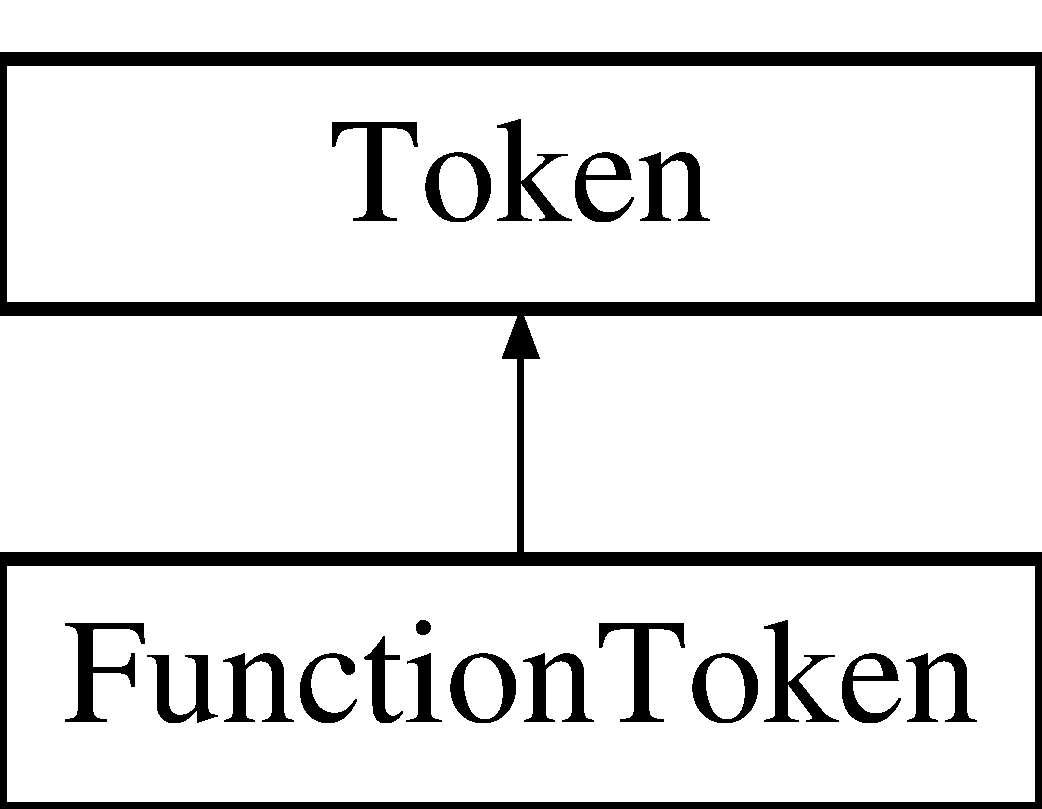
\includegraphics[height=2.000000cm]{classFunctionToken}
\end{center}
\end{figure}
\subsection*{Public Types}
\begin{DoxyCompactItemize}
\item 
enum {\bfseries Function\-Id} \{ {\bfseries Exponential}, 
{\bfseries Square\-Root}, 
{\bfseries Factorial}
 \}
\end{DoxyCompactItemize}
\subsection*{Public Member Functions}
\begin{DoxyCompactItemize}
\item 
\hypertarget{classFunctionToken_a5ee4a06cd8e2a8a7e5edaacd584a4c35}{{\bfseries Function\-Token} (Function\-Id function\-Id)}\label{classFunctionToken_a5ee4a06cd8e2a8a7e5edaacd584a4c35}

\item 
\hypertarget{classFunctionToken_abc4e12e95528a717d397e9e2fff1d67f}{virtual \hyperlink{classFunctionToken}{Function\-Token} $\ast$ {\bfseries clone} () const }\label{classFunctionToken_abc4e12e95528a717d397e9e2fff1d67f}

\item 
\hypertarget{classFunctionToken_ad34c535630da433a40dd68388e610aee}{Function\-Id {\bfseries function\-Id} () const }\label{classFunctionToken_ad34c535630da433a40dd68388e610aee}

\item 
\hypertarget{classFunctionToken_a43b402da5b91e0aaca01a99e4a2543c3}{unsigned int {\bfseries param\-Num} () const }\label{classFunctionToken_a43b402da5b91e0aaca01a99e4a2543c3}

\end{DoxyCompactItemize}


The documentation for this class was generated from the following files\-:\begin{DoxyCompactItemize}
\item 
inc/core/\hyperlink{token_8h}{token.\-h}\item 
src/core/\hyperlink{token_8cpp}{token.\-cpp}\end{DoxyCompactItemize}

\hypertarget{classLexicalException}{\section{Lexical\-Exception Class Reference}
\label{classLexicalException}\index{Lexical\-Exception@{Lexical\-Exception}}
}
Inheritance diagram for Lexical\-Exception\-:\begin{figure}[H]
\begin{center}
\leavevmode
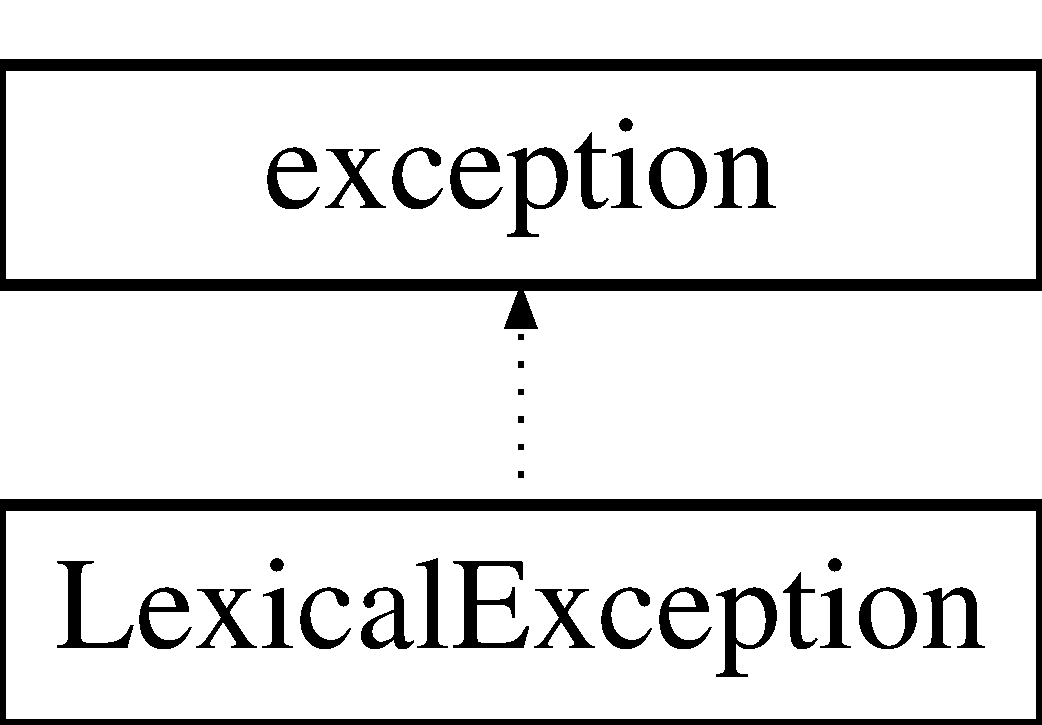
\includegraphics[height=2.000000cm]{classLexicalException}
\end{center}
\end{figure}


The documentation for this class was generated from the following file\-:\begin{DoxyCompactItemize}
\item 
inc/core/\hyperlink{myexception_8h}{myexception.\-h}\end{DoxyCompactItemize}

\hypertarget{classMainWindow}{\section{Main\-Window Class Reference}
\label{classMainWindow}\index{Main\-Window@{Main\-Window}}
}
Inheritance diagram for Main\-Window\-:\begin{figure}[H]
\begin{center}
\leavevmode
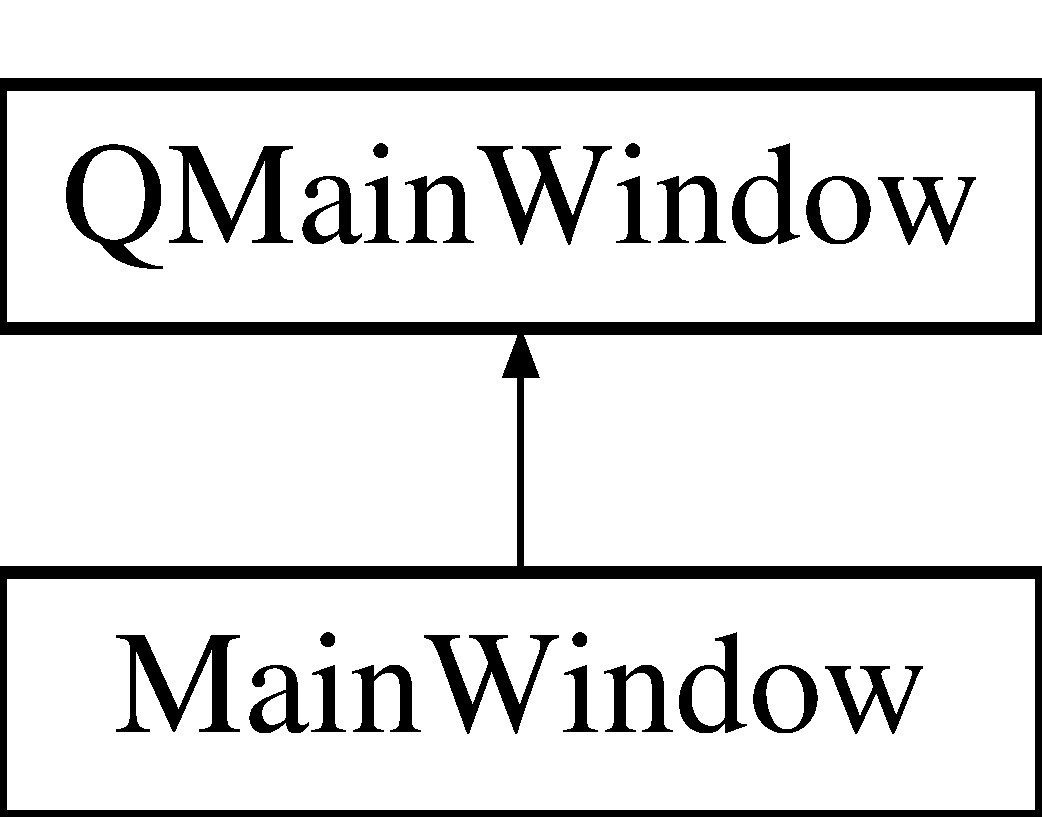
\includegraphics[height=2.000000cm]{classMainWindow}
\end{center}
\end{figure}
\subsection*{Public Member Functions}
\begin{DoxyCompactItemize}
\item 
\hypertarget{classMainWindow_a8b244be8b7b7db1b08de2a2acb9409db}{{\bfseries Main\-Window} (Q\-Widget $\ast$parent=0)}\label{classMainWindow_a8b244be8b7b7db1b08de2a2acb9409db}

\end{DoxyCompactItemize}
\subsection*{Public Attributes}
\begin{DoxyCompactItemize}
\item 
\hypertarget{classMainWindow_a624a009d3c1cc1a8f1ab586f09e8bc01}{Q\-String {\bfseries example}}\label{classMainWindow_a624a009d3c1cc1a8f1ab586f09e8bc01}

\end{DoxyCompactItemize}


The documentation for this class was generated from the following files\-:\begin{DoxyCompactItemize}
\item 
inc/gui/\hyperlink{mainwindow_8h}{mainwindow.\-h}\item 
src/gui/mainwindow.\-cpp\end{DoxyCompactItemize}

\hypertarget{classMath}{\section{Math Class Reference}
\label{classMath}\index{Math@{Math}}
}
\subsection*{Static Public Member Functions}
\begin{DoxyCompactItemize}
\item 
static double \hyperlink{classMath_ac9774c99a4f12bb928f1d59483a62f55}{add} (double a, double b)
\item 
static double \hyperlink{classMath_a6b48894bada3b49a788dd9050bbe29ee}{sub} (double a, double b)
\item 
static double \hyperlink{classMath_a2960dd27ba97e81da9b99e4f3de9231f}{mul} (double a, double b)
\item 
static double \hyperlink{classMath_aa8d168d849ae9be946f5d8ec2d0db39e}{div} (double a, double b)
\item 
static double \hyperlink{classMath_a1f660660916446dd095fe40cfaaccd45}{exp} (double x, int exp)
\item 
static double \hyperlink{classMath_a79979f796703a578f12c95517812466e}{sqrt} (double x)
\item 
static int \hyperlink{classMath_a88c1cd28a6edb1959d062fc477d61d31}{fact} (int x)
\item 
static double \hyperlink{classMath_a496de1930a0299faa8d40d681ef4301e}{abs} (double x)
\end{DoxyCompactItemize}


\subsection{Member Function Documentation}
\hypertarget{classMath_a496de1930a0299faa8d40d681ef4301e}{\index{Math@{Math}!abs@{abs}}
\index{abs@{abs}!Math@{Math}}
\subsubsection[{abs}]{\setlength{\rightskip}{0pt plus 5cm}double Math\-::abs (
\begin{DoxyParamCaption}
\item[{double}]{x}
\end{DoxyParamCaption}
)\hspace{0.3cm}{\ttfamily [static]}}}\label{classMath_a496de1930a0299faa8d40d681ef4301e}
Absolute value of number 
\begin{DoxyParams}{Parameters}
{\em x} & number \\
\hline
\end{DoxyParams}
\begin{DoxyReturn}{Returns}
result of operation 
\end{DoxyReturn}
\hypertarget{classMath_ac9774c99a4f12bb928f1d59483a62f55}{\index{Math@{Math}!add@{add}}
\index{add@{add}!Math@{Math}}
\subsubsection[{add}]{\setlength{\rightskip}{0pt plus 5cm}double Math\-::add (
\begin{DoxyParamCaption}
\item[{double}]{a, }
\item[{double}]{b}
\end{DoxyParamCaption}
)\hspace{0.3cm}{\ttfamily [static]}}}\label{classMath_ac9774c99a4f12bb928f1d59483a62f55}
Adding two numbers 
\begin{DoxyParams}{Parameters}
{\em a} & first number \\
\hline
{\em b} & second number \\
\hline
\end{DoxyParams}
\begin{DoxyReturn}{Returns}
result of operation 
\end{DoxyReturn}
\hypertarget{classMath_aa8d168d849ae9be946f5d8ec2d0db39e}{\index{Math@{Math}!div@{div}}
\index{div@{div}!Math@{Math}}
\subsubsection[{div}]{\setlength{\rightskip}{0pt plus 5cm}double Math\-::div (
\begin{DoxyParamCaption}
\item[{double}]{a, }
\item[{double}]{b}
\end{DoxyParamCaption}
)\hspace{0.3cm}{\ttfamily [static]}}}\label{classMath_aa8d168d849ae9be946f5d8ec2d0db39e}
Divide two numbers 
\begin{DoxyParams}{Parameters}
{\em a} & first number \\
\hline
{\em b} & second number \\
\hline
\end{DoxyParams}

\begin{DoxyExceptions}{Exceptions}
{\em \hyperlink{classMathException}{Math\-Exception}} & divided by zero \\
\hline
\end{DoxyExceptions}
\begin{DoxyReturn}{Returns}
result of operation 
\end{DoxyReturn}
\hypertarget{classMath_a1f660660916446dd095fe40cfaaccd45}{\index{Math@{Math}!exp@{exp}}
\index{exp@{exp}!Math@{Math}}
\subsubsection[{exp}]{\setlength{\rightskip}{0pt plus 5cm}double Math\-::exp (
\begin{DoxyParamCaption}
\item[{double}]{x, }
\item[{int}]{exp}
\end{DoxyParamCaption}
)\hspace{0.3cm}{\ttfamily [static]}}}\label{classMath_a1f660660916446dd095fe40cfaaccd45}
Squaring number 
\begin{DoxyParams}{Parameters}
{\em x} & number \\
\hline
{\em exp} & exponent \\
\hline
\end{DoxyParams}
\begin{DoxyReturn}{Returns}
result of operation 
\end{DoxyReturn}
\hypertarget{classMath_a88c1cd28a6edb1959d062fc477d61d31}{\index{Math@{Math}!fact@{fact}}
\index{fact@{fact}!Math@{Math}}
\subsubsection[{fact}]{\setlength{\rightskip}{0pt plus 5cm}int Math\-::fact (
\begin{DoxyParamCaption}
\item[{int}]{x}
\end{DoxyParamCaption}
)\hspace{0.3cm}{\ttfamily [static]}}}\label{classMath_a88c1cd28a6edb1959d062fc477d61d31}
Factorial of number 
\begin{DoxyParams}{Parameters}
{\em x} & number \\
\hline
\end{DoxyParams}
\begin{DoxyReturn}{Returns}
result of operation 
\end{DoxyReturn}
\hypertarget{classMath_a2960dd27ba97e81da9b99e4f3de9231f}{\index{Math@{Math}!mul@{mul}}
\index{mul@{mul}!Math@{Math}}
\subsubsection[{mul}]{\setlength{\rightskip}{0pt plus 5cm}double Math\-::mul (
\begin{DoxyParamCaption}
\item[{double}]{a, }
\item[{double}]{b}
\end{DoxyParamCaption}
)\hspace{0.3cm}{\ttfamily [static]}}}\label{classMath_a2960dd27ba97e81da9b99e4f3de9231f}
Multiply two numbers 
\begin{DoxyParams}{Parameters}
{\em a} & first number \\
\hline
{\em b} & second number \\
\hline
\end{DoxyParams}
\begin{DoxyReturn}{Returns}
result of operation 
\end{DoxyReturn}
\hypertarget{classMath_a79979f796703a578f12c95517812466e}{\index{Math@{Math}!sqrt@{sqrt}}
\index{sqrt@{sqrt}!Math@{Math}}
\subsubsection[{sqrt}]{\setlength{\rightskip}{0pt plus 5cm}double Math\-::sqrt (
\begin{DoxyParamCaption}
\item[{double}]{x}
\end{DoxyParamCaption}
)\hspace{0.3cm}{\ttfamily [static]}}}\label{classMath_a79979f796703a578f12c95517812466e}
The square root of number 
\begin{DoxyParams}{Parameters}
{\em x} & number \\
\hline
\end{DoxyParams}
\begin{DoxyReturn}{Returns}
result of operation 
\end{DoxyReturn}
\hypertarget{classMath_a6b48894bada3b49a788dd9050bbe29ee}{\index{Math@{Math}!sub@{sub}}
\index{sub@{sub}!Math@{Math}}
\subsubsection[{sub}]{\setlength{\rightskip}{0pt plus 5cm}double Math\-::sub (
\begin{DoxyParamCaption}
\item[{double}]{a, }
\item[{double}]{b}
\end{DoxyParamCaption}
)\hspace{0.3cm}{\ttfamily [static]}}}\label{classMath_a6b48894bada3b49a788dd9050bbe29ee}
Subtraction of two numbers 
\begin{DoxyParams}{Parameters}
{\em a} & first number \\
\hline
{\em b} & second number \\
\hline
\end{DoxyParams}
\begin{DoxyReturn}{Returns}
result of operation 
\end{DoxyReturn}


The documentation for this class was generated from the following files\-:\begin{DoxyCompactItemize}
\item 
inc/core/\hyperlink{math_8h}{math.\-h}\item 
src/core/\hyperlink{math_8cpp}{math.\-cpp}\end{DoxyCompactItemize}

\hypertarget{classMathException}{\section{Math\-Exception Class Reference}
\label{classMathException}\index{Math\-Exception@{Math\-Exception}}
}
Inheritance diagram for Math\-Exception\-:\begin{figure}[H]
\begin{center}
\leavevmode
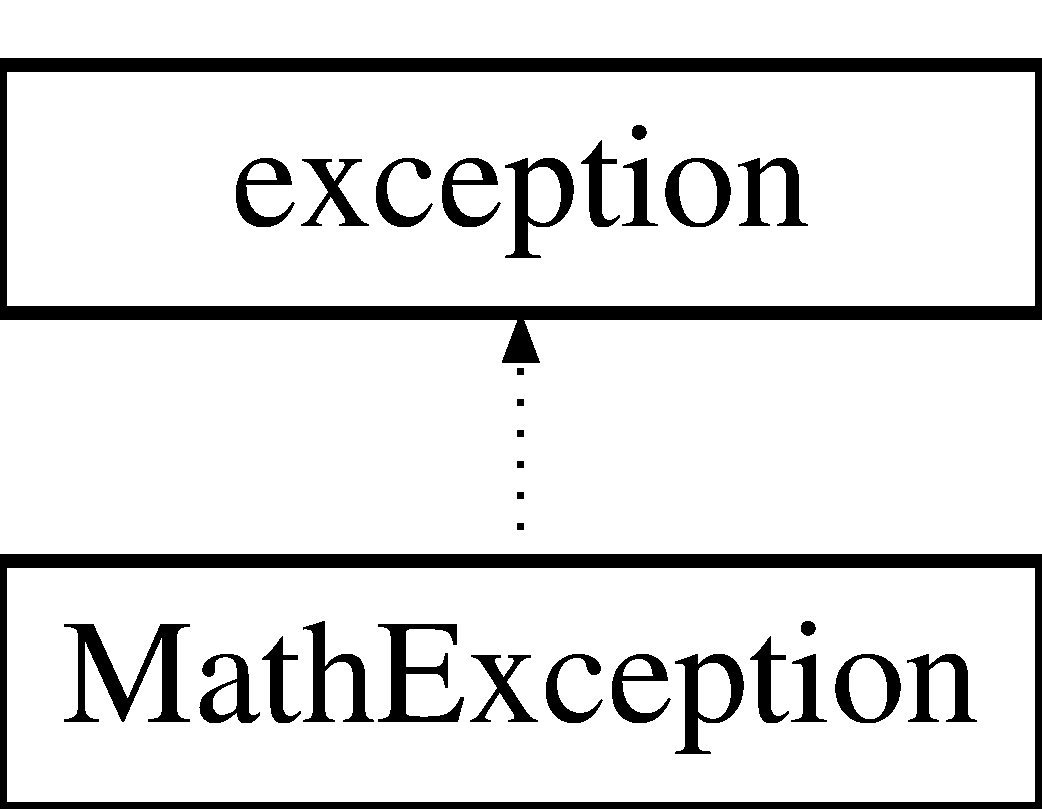
\includegraphics[height=2.000000cm]{classMathException}
\end{center}
\end{figure}


The documentation for this class was generated from the following file\-:\begin{DoxyCompactItemize}
\item 
inc/core/\hyperlink{myexception_8h}{myexception.\-h}\end{DoxyCompactItemize}

\hypertarget{classmathTestHeader}{\section{math\-Test\-Header Class Reference}
\label{classmathTestHeader}\index{math\-Test\-Header@{math\-Test\-Header}}
}
Inheritance diagram for math\-Test\-Header\-:\begin{figure}[H]
\begin{center}
\leavevmode
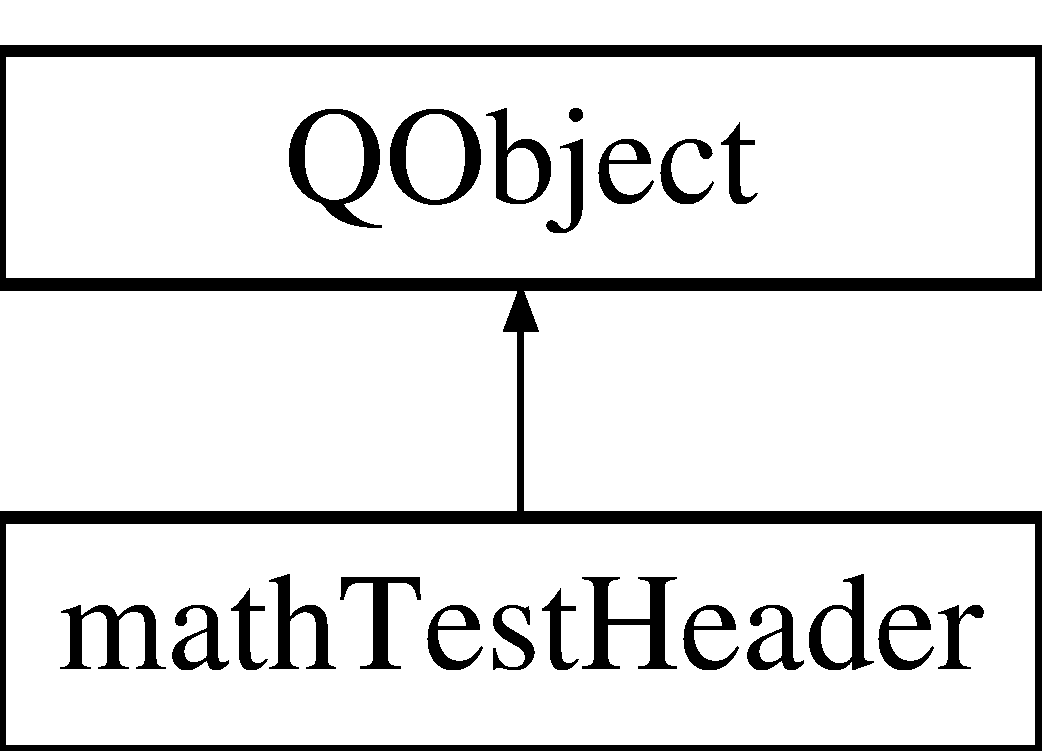
\includegraphics[height=2.000000cm]{classmathTestHeader}
\end{center}
\end{figure}


The documentation for this class was generated from the following files\-:\begin{DoxyCompactItemize}
\item 
inc/tests/\hyperlink{mathTestHeader_8h}{math\-Test\-Header.\-h}\item 
src/tests/\hyperlink{mathTest_8cpp}{math\-Test.\-cpp}\end{DoxyCompactItemize}

\hypertarget{classNumberToken}{\section{Number\-Token Class Reference}
\label{classNumberToken}\index{Number\-Token@{Number\-Token}}
}
Inheritance diagram for Number\-Token\-:\begin{figure}[H]
\begin{center}
\leavevmode
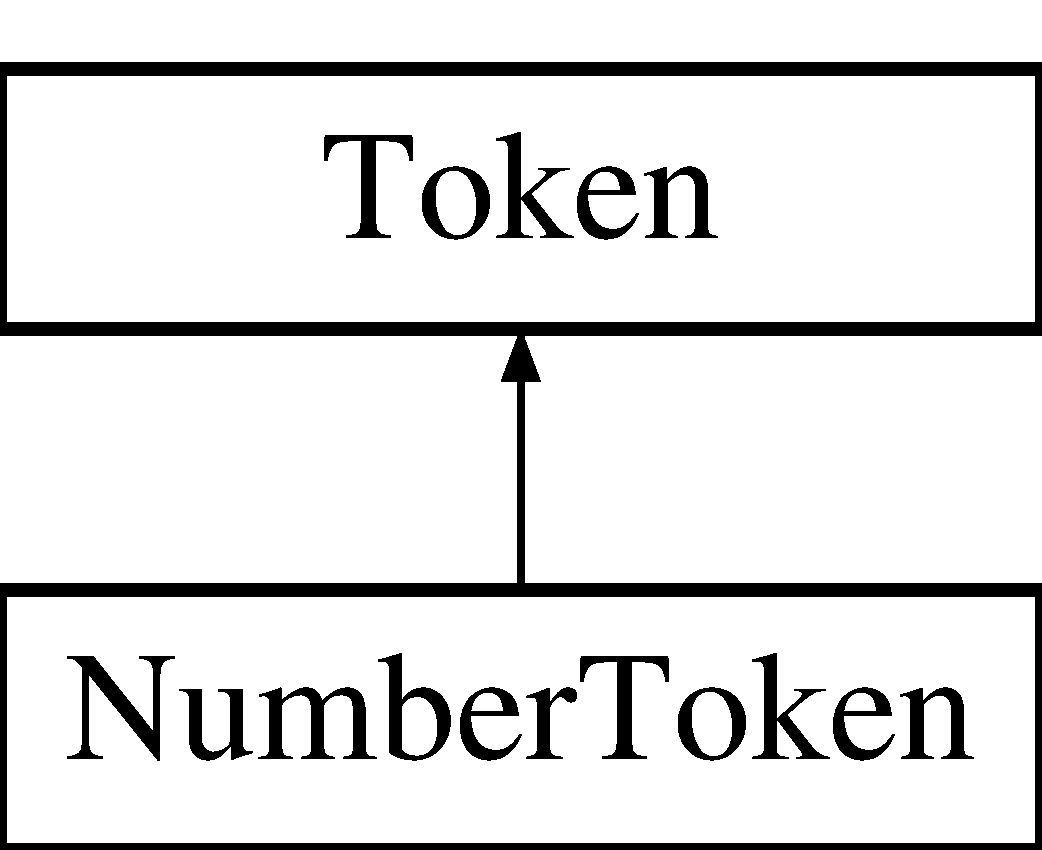
\includegraphics[height=2.000000cm]{classNumberToken}
\end{center}
\end{figure}
\subsection*{Public Member Functions}
\begin{DoxyCompactItemize}
\item 
\hypertarget{classNumberToken_a2b6ffba5b946b47d6c8ed7152bce78e9}{{\bfseries Number\-Token} (double number)}\label{classNumberToken_a2b6ffba5b946b47d6c8ed7152bce78e9}

\item 
\hypertarget{classNumberToken_a6d52d4b69c1fa1f5cbd182bf6f889d08}{virtual \hyperlink{classNumberToken}{Number\-Token} $\ast$ {\bfseries clone} () const }\label{classNumberToken_a6d52d4b69c1fa1f5cbd182bf6f889d08}

\item 
\hypertarget{classNumberToken_a5caf616bb2eaf58958cc04a8db99d705}{double {\bfseries number} () const }\label{classNumberToken_a5caf616bb2eaf58958cc04a8db99d705}

\item 
\hypertarget{classNumberToken_a52a2337c677a57fcd25df5c2d343d8d1}{void {\bfseries number} (double number)}\label{classNumberToken_a52a2337c677a57fcd25df5c2d343d8d1}

\end{DoxyCompactItemize}
\subsection*{Additional Inherited Members}


The documentation for this class was generated from the following files\-:\begin{DoxyCompactItemize}
\item 
inc/core/\hyperlink{token_8h}{token.\-h}\item 
src/core/\hyperlink{token_8cpp}{token.\-cpp}\end{DoxyCompactItemize}

\hypertarget{classParser}{\section{Parser Class Reference}
\label{classParser}\index{Parser@{Parser}}
}
\subsection*{Public Member Functions}
\begin{DoxyCompactItemize}
\item 
double \hyperlink{classParser_a95aea0181f7451feb9e98ac8e97cb59d}{parse} (\hyperlink{classTokenVector}{Token\-Vector} \&token\-Vector)
\end{DoxyCompactItemize}


\subsection{Member Function Documentation}
\hypertarget{classParser_a95aea0181f7451feb9e98ac8e97cb59d}{\index{Parser@{Parser}!parse@{parse}}
\index{parse@{parse}!Parser@{Parser}}
\subsubsection[{parse}]{\setlength{\rightskip}{0pt plus 5cm}double Parser\-::parse (
\begin{DoxyParamCaption}
\item[{{\bf Token\-Vector} \&}]{token\-Vector}
\end{DoxyParamCaption}
)}}\label{classParser_a95aea0181f7451feb9e98ac8e97cb59d}
Main function of parser 
\begin{DoxyParams}{Parameters}
{\em token\-Vector} & vector of tokens (\hyperlink{classToken}{Token} class) \\
\hline
\end{DoxyParams}

\begin{DoxyExceptions}{Exceptions}
{\em \hyperlink{classSyntaxException}{Syntax\-Exception}} & wrong expression \\
\hline
\end{DoxyExceptions}
\begin{DoxyReturn}{Returns}
mathematical result 
\end{DoxyReturn}


The documentation for this class was generated from the following files\-:\begin{DoxyCompactItemize}
\item 
inc/core/\hyperlink{parser_8h}{parser.\-h}\item 
src/core/\hyperlink{parser_8cpp}{parser.\-cpp}\end{DoxyCompactItemize}

\hypertarget{classScanner}{\section{Scanner Class Reference}
\label{classScanner}\index{Scanner@{Scanner}}
}
\subsection*{Public Member Functions}
\begin{DoxyCompactItemize}
\item 
\hyperlink{classTokenVector}{Token\-Vector} \hyperlink{classScanner_a64edbc407f889927bd871a962f9db893}{scan} (std\-::string input)
\end{DoxyCompactItemize}


\subsection{Member Function Documentation}
\hypertarget{classScanner_a64edbc407f889927bd871a962f9db893}{\index{Scanner@{Scanner}!scan@{scan}}
\index{scan@{scan}!Scanner@{Scanner}}
\subsubsection[{scan}]{\setlength{\rightskip}{0pt plus 5cm}{\bf Token\-Vector} Scanner\-::scan (
\begin{DoxyParamCaption}
\item[{std\-::string}]{input}
\end{DoxyParamCaption}
)}}\label{classScanner_a64edbc407f889927bd871a962f9db893}
Scans expression and creates tokens 
\begin{DoxyParams}{Parameters}
{\em input} & expression \\
\hline
\end{DoxyParams}

\begin{DoxyExceptions}{Exceptions}
{\em \hyperlink{classLexicalException}{Lexical\-Exception}} & wrong expression \\
\hline
\end{DoxyExceptions}
\begin{DoxyReturn}{Returns}
token\-Vector vector of tokens 
\end{DoxyReturn}


The documentation for this class was generated from the following files\-:\begin{DoxyCompactItemize}
\item 
inc/core/\hyperlink{scanner_8h}{scanner.\-h}\item 
src/core/\hyperlink{scanner_8cpp}{scanner.\-cpp}\end{DoxyCompactItemize}

\hypertarget{classSyntaxException}{\section{Syntax\-Exception Class Reference}
\label{classSyntaxException}\index{Syntax\-Exception@{Syntax\-Exception}}
}
Inheritance diagram for Syntax\-Exception\-:\begin{figure}[H]
\begin{center}
\leavevmode
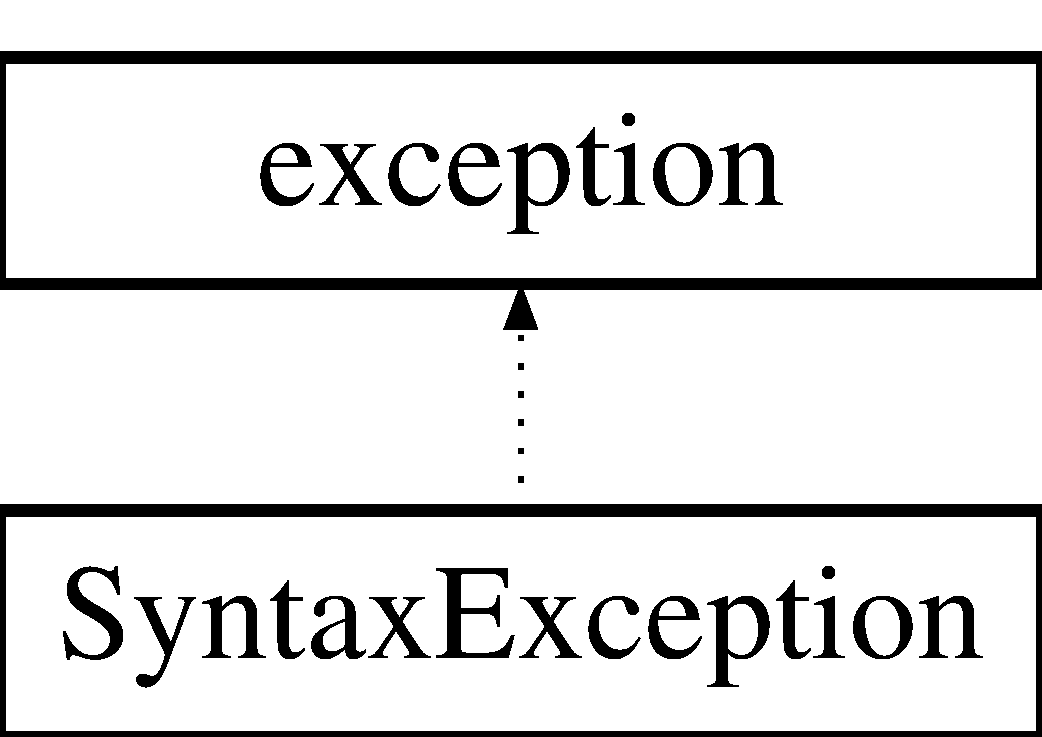
\includegraphics[height=2.000000cm]{classSyntaxException}
\end{center}
\end{figure}


The documentation for this class was generated from the following file\-:\begin{DoxyCompactItemize}
\item 
inc/core/\hyperlink{myexception_8h}{myexception.\-h}\end{DoxyCompactItemize}

\hypertarget{classToken}{\section{Token Class Reference}
\label{classToken}\index{Token@{Token}}
}
Inheritance diagram for Token\-:\begin{figure}[H]
\begin{center}
\leavevmode
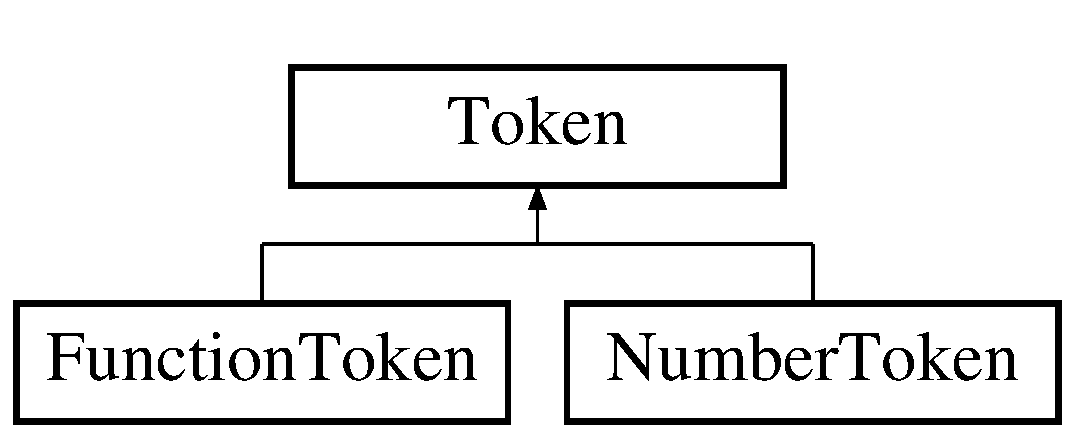
\includegraphics[height=2.000000cm]{classToken}
\end{center}
\end{figure}
\subsection*{Public Types}
\begin{DoxyCompactItemize}
\item 
enum {\bfseries Type} \{ \\*
{\bfseries Number}, 
{\bfseries Function}, 
{\bfseries Left\-Brace}, 
{\bfseries Right\-Brace}, 
\\*
{\bfseries Comma}, 
{\bfseries Plus}, 
{\bfseries Minus}, 
{\bfseries Multiply}, 
\\*
{\bfseries Divide}, 
{\bfseries Exp}, 
{\bfseries End}
 \}
\end{DoxyCompactItemize}
\subsection*{Public Member Functions}
\begin{DoxyCompactItemize}
\item 
\hypertarget{classToken_ac5b1af731830b70f07e948c466becf5e}{{\bfseries Token} (Type type)}\label{classToken_ac5b1af731830b70f07e948c466becf5e}

\item 
\hypertarget{classToken_a3ae2969e35156789ddd09ee0843caca1}{virtual \hyperlink{classToken}{Token} $\ast$ {\bfseries clone} () const }\label{classToken_a3ae2969e35156789ddd09ee0843caca1}

\item 
\hypertarget{classToken_a3fea7300d8391a3da7a3a5bc63969d0d}{Type {\bfseries type} () const }\label{classToken_a3fea7300d8391a3da7a3a5bc63969d0d}

\item 
\hypertarget{classToken_a97ed582c3ba469e23266a1d8fb7229ee}{bool {\bfseries skip} ()}\label{classToken_a97ed582c3ba469e23266a1d8fb7229ee}

\item 
\hypertarget{classToken_a7017ff7cd24c4cd05af0cb654ecde369}{bool {\bfseries is\-Skipped} ()}\label{classToken_a7017ff7cd24c4cd05af0cb654ecde369}

\end{DoxyCompactItemize}


The documentation for this class was generated from the following files\-:\begin{DoxyCompactItemize}
\item 
inc/core/\hyperlink{token_8h}{token.\-h}\item 
src/core/\hyperlink{token_8cpp}{token.\-cpp}\end{DoxyCompactItemize}

\hypertarget{classTokenVector}{\section{Token\-Vector Class Reference}
\label{classTokenVector}\index{Token\-Vector@{Token\-Vector}}
}
\subsection*{Public Member Functions}
\begin{DoxyCompactItemize}
\item 
\hypertarget{classTokenVector_ae2103ba63c116b1837d425443a5ce48d}{{\bfseries Token\-Vector} (const \hyperlink{classTokenVector}{Token\-Vector} \&other)}\label{classTokenVector_ae2103ba63c116b1837d425443a5ce48d}

\item 
\hypertarget{classTokenVector_a9adbc1cf57a958a8eb52430f7e205f91}{\hyperlink{classToken}{Token} $\ast$ {\bfseries operator\mbox{[}$\,$\mbox{]}} (std\-::vector$<$ \hyperlink{classToken}{Token} $\ast$ $>$\-::size\-\_\-type idx) const }\label{classTokenVector_a9adbc1cf57a958a8eb52430f7e205f91}

\item 
\hypertarget{classTokenVector_aaddb50ad038adf29571e273f7d92641f}{std\-::vector$<$ \hyperlink{classToken}{Token} $\ast$ $>$\-::size\-\_\-type {\bfseries size} () const }\label{classTokenVector_aaddb50ad038adf29571e273f7d92641f}

\item 
\hypertarget{classTokenVector_aa9864c6f20c4126c37412b74f6ab08e9}{void {\bfseries add} (\hyperlink{classToken}{Token} $\ast$token)}\label{classTokenVector_aa9864c6f20c4126c37412b74f6ab08e9}

\end{DoxyCompactItemize}


The documentation for this class was generated from the following files\-:\begin{DoxyCompactItemize}
\item 
inc/core/\hyperlink{token_8h}{token.\-h}\item 
src/core/\hyperlink{token_8cpp}{token.\-cpp}\end{DoxyCompactItemize}

\chapter{File Documentation}
\hypertarget{math_8h}{\section{inc/core/math.h File Reference}
\label{math_8h}\index{inc/core/math.\-h@{inc/core/math.\-h}}
}


math \hyperlink{math_8cpp}{math.\-cpp}  


{\ttfamily \#include $<$stdexcept$>$}\\*
\subsection*{Classes}
\begin{DoxyCompactItemize}
\item 
class \hyperlink{classMath}{Math}
\end{DoxyCompactItemize}


\subsection{Detailed Description}
math \hyperlink{math_8cpp}{math.\-cpp} \begin{DoxyAuthor}{Author}
Tomas Polesovsky, Miroslav Pavelek, Ivan Sevcik, Zdenek Sklenar 
\end{DoxyAuthor}

\hypertarget{myexception_8h}{\section{inc/core/myexception.h File Reference}
\label{myexception_8h}\index{inc/core/myexception.\-h@{inc/core/myexception.\-h}}
}


myexception myexception.\-cpp  


{\ttfamily \#include $<$stdexcept$>$}\\*
\subsection*{Classes}
\begin{DoxyCompactItemize}
\item 
class \hyperlink{classMathException}{Math\-Exception}
\item 
class \hyperlink{classLexicalException}{Lexical\-Exception}
\item 
class \hyperlink{classSyntaxException}{Syntax\-Exception}
\end{DoxyCompactItemize}


\subsection{Detailed Description}
myexception myexception.\-cpp \begin{DoxyAuthor}{Author}
Tomas Polesovsky, Miroslav Pavelek, Ivan Sevcik, Zdenek Sklenar 
\end{DoxyAuthor}

\hypertarget{parser_8h}{\section{inc/core/parser.h File Reference}
\label{parser_8h}\index{inc/core/parser.\-h@{inc/core/parser.\-h}}
}


parser \hyperlink{parser_8cpp}{parser.\-cpp}  


{\ttfamily \#include \char`\"{}token.\-h\char`\"{}}\\*
{\ttfamily \#include $<$cstdint$>$}\\*
{\ttfamily \#include $<$vector$>$}\\*
\subsection*{Classes}
\begin{DoxyCompactItemize}
\item 
class \hyperlink{classParser}{Parser}
\end{DoxyCompactItemize}


\subsection{Detailed Description}
parser \hyperlink{parser_8cpp}{parser.\-cpp} \begin{DoxyAuthor}{Author}
Tomas Polesovsky, Miroslav Pavelek, Ivan Sevcik, Zdenek Sklenar 
\end{DoxyAuthor}

\hypertarget{scanner_8h}{\section{inc/core/scanner.h File Reference}
\label{scanner_8h}\index{inc/core/scanner.\-h@{inc/core/scanner.\-h}}
}


scanner \hyperlink{scanner_8cpp}{scanner.\-cpp}  


{\ttfamily \#include $<$vector$>$}\\*
{\ttfamily \#include $<$string$>$}\\*
{\ttfamily \#include $<$stdexcept$>$}\\*
{\ttfamily \#include \char`\"{}token.\-h\char`\"{}}\\*
\subsection*{Classes}
\begin{DoxyCompactItemize}
\item 
class \hyperlink{classScanner}{Scanner}
\end{DoxyCompactItemize}


\subsection{Detailed Description}
scanner \hyperlink{scanner_8cpp}{scanner.\-cpp} \begin{DoxyAuthor}{Author}
Tomas Polesovsky, Miroslav Pavelek, Ivan Sevcik, Zdenek Sklenar 
\end{DoxyAuthor}

\hypertarget{token_8h}{\section{inc/core/token.h File Reference}
\label{token_8h}\index{inc/core/token.\-h@{inc/core/token.\-h}}
}


token \hyperlink{token_8cpp}{token.\-cpp}  


{\ttfamily \#include $<$vector$>$}\\*
\subsection*{Classes}
\begin{DoxyCompactItemize}
\item 
class \hyperlink{classToken}{Token}
\item 
class \hyperlink{classNumberToken}{Number\-Token}
\item 
class \hyperlink{classFunctionToken}{Function\-Token}
\item 
class \hyperlink{classTokenVector}{Token\-Vector}
\end{DoxyCompactItemize}


\subsection{Detailed Description}
token \hyperlink{token_8cpp}{token.\-cpp} \begin{DoxyAuthor}{Author}
Tomas Polesovsky, Miroslav Pavelek, Ivan Sevcik, Zdenek Sklenar 
\end{DoxyAuthor}

\hypertarget{mainwindow_8h}{\section{inc/gui/mainwindow.h File Reference}
\label{mainwindow_8h}\index{inc/gui/mainwindow.\-h@{inc/gui/mainwindow.\-h}}
}


mainwindow mainwindow.\-cpp  


{\ttfamily \#include $<$Q\-Main\-Window$>$}\\*
{\ttfamily \#include $<$Q\-Message\-Box$>$}\\*
\subsection*{Classes}
\begin{DoxyCompactItemize}
\item 
class \hyperlink{classMainWindow}{Main\-Window}
\end{DoxyCompactItemize}


\subsection{Detailed Description}
mainwindow mainwindow.\-cpp \begin{DoxyAuthor}{Author}
Tomas Polesovsky, Miroslav Pavelek, Ivan Sevcik, Zdenek Sklenar 
\end{DoxyAuthor}

\hypertarget{mathTestHeader_8h}{\section{inc/tests/math\-Test\-Header.h File Reference}
\label{mathTestHeader_8h}\index{inc/tests/math\-Test\-Header.\-h@{inc/tests/math\-Test\-Header.\-h}}
}


\hyperlink{classmathTestHeader}{math\-Test\-Header} math\-Test\-Header.\-cpp  


{\ttfamily \#include $<$Q\-Object$>$}\\*
\subsection*{Classes}
\begin{DoxyCompactItemize}
\item 
class \hyperlink{classmathTestHeader}{math\-Test\-Header}
\end{DoxyCompactItemize}


\subsection{Detailed Description}
\hyperlink{classmathTestHeader}{math\-Test\-Header} math\-Test\-Header.\-cpp \begin{DoxyAuthor}{Author}
Tomas Polesovsky, Miroslav Pavelek, Ivan Sevcik, Zdenek Sklenar 
\end{DoxyAuthor}

\hypertarget{math_8cpp}{\section{src/core/math.cpp File Reference}
\label{math_8cpp}\index{src/core/math.\-cpp@{src/core/math.\-cpp}}
}


Mathematical library including primary operations and functions.  


{\ttfamily \#include \char`\"{}inc/core/math.\-h\char`\"{}}\\*
{\ttfamily \#include \char`\"{}inc/core/myexception.\-h\char`\"{}}\\*


\subsection{Detailed Description}
Mathematical library including primary operations and functions. \begin{DoxyAuthor}{Author}
Tomas Polesovsky, Miroslav Pavelek, Ivan Sevcik, Zdenek Sklenar 
\end{DoxyAuthor}

\hypertarget{parser_8cpp}{\section{src/core/parser.cpp File Reference}
\label{parser_8cpp}\index{src/core/parser.\-cpp@{src/core/parser.\-cpp}}
}


Syntactic analysis.  


{\ttfamily \#include \char`\"{}inc/core/parser.\-h\char`\"{}}\\*
{\ttfamily \#include \char`\"{}inc/core/token.\-h\char`\"{}}\\*
{\ttfamily \#include $<$stdexcept$>$}\\*
{\ttfamily \#include \char`\"{}inc/core/math.\-h\char`\"{}}\\*
{\ttfamily \#include \char`\"{}inc/core/myexception.\-h\char`\"{}}\\*
\subsection*{Enumerations}
\begin{DoxyCompactItemize}
\item 
enum \hyperlink{parser_8cpp_aba2a120c4cddd8d30aee80f6c7f1872b}{Token\-Precedence} \{ \hyperlink{parser_8cpp_aba2a120c4cddd8d30aee80f6c7f1872ba7a352a3dd2accc1dd65a4538c3754ee8}{Low}, 
\hyperlink{parser_8cpp_aba2a120c4cddd8d30aee80f6c7f1872ba24c57acd029e3f96fede49402ea01e6f}{High}, 
\hyperlink{parser_8cpp_aba2a120c4cddd8d30aee80f6c7f1872ba4c2ccc0164cc7fc1102a4b69361acd1e}{Equal}, 
\hyperlink{parser_8cpp_aba2a120c4cddd8d30aee80f6c7f1872ba4dfd42ec49d09d8c6555c218301cc30f}{Error}
 \}
\end{DoxyCompactItemize}


\subsection{Detailed Description}
Syntactic analysis. \begin{DoxyAuthor}{Author}
Tomas Polesovsky, Miroslav Pavelek, Ivan Sevcik, Zdenek Sklenar 
\end{DoxyAuthor}


\subsection{Enumeration Type Documentation}
\hypertarget{parser_8cpp_aba2a120c4cddd8d30aee80f6c7f1872b}{\index{parser.\-cpp@{parser.\-cpp}!Token\-Precedence@{Token\-Precedence}}
\index{Token\-Precedence@{Token\-Precedence}!parser.cpp@{parser.\-cpp}}
\subsubsection[{Token\-Precedence}]{\setlength{\rightskip}{0pt plus 5cm}enum {\bf Token\-Precedence}}}\label{parser_8cpp_aba2a120c4cddd8d30aee80f6c7f1872b}
\begin{Desc}
\item[Enumerator]\par
\begin{description}
\index{Low@{Low}!parser.\-cpp@{parser.\-cpp}}\index{parser.\-cpp@{parser.\-cpp}!Low@{Low}}\item[{\em 
\hypertarget{parser_8cpp_aba2a120c4cddd8d30aee80f6c7f1872ba7a352a3dd2accc1dd65a4538c3754ee8}{Low}\label{parser_8cpp_aba2a120c4cddd8d30aee80f6c7f1872ba7a352a3dd2accc1dd65a4538c3754ee8}
}]\hyperlink{classToken}{Token} on the top of the stack has lower priority than input token. \index{High@{High}!parser.\-cpp@{parser.\-cpp}}\index{parser.\-cpp@{parser.\-cpp}!High@{High}}\item[{\em 
\hypertarget{parser_8cpp_aba2a120c4cddd8d30aee80f6c7f1872ba24c57acd029e3f96fede49402ea01e6f}{High}\label{parser_8cpp_aba2a120c4cddd8d30aee80f6c7f1872ba24c57acd029e3f96fede49402ea01e6f}
}]\hyperlink{classToken}{Token} on the top of the stack has higher priority than input token. \index{Equal@{Equal}!parser.\-cpp@{parser.\-cpp}}\index{parser.\-cpp@{parser.\-cpp}!Equal@{Equal}}\item[{\em 
\hypertarget{parser_8cpp_aba2a120c4cddd8d30aee80f6c7f1872ba4c2ccc0164cc7fc1102a4b69361acd1e}{Equal}\label{parser_8cpp_aba2a120c4cddd8d30aee80f6c7f1872ba4c2ccc0164cc7fc1102a4b69361acd1e}
}]\hyperlink{classToken}{Token} on the top of the stack has same priority as input token. \index{Error@{Error}!parser.\-cpp@{parser.\-cpp}}\index{parser.\-cpp@{parser.\-cpp}!Error@{Error}}\item[{\em 
\hypertarget{parser_8cpp_aba2a120c4cddd8d30aee80f6c7f1872ba4dfd42ec49d09d8c6555c218301cc30f}{Error}\label{parser_8cpp_aba2a120c4cddd8d30aee80f6c7f1872ba4dfd42ec49d09d8c6555c218301cc30f}
}]\hyperlink{classToken}{Token} on the top of the stack cannot be followed by input token, syntax error. \end{description}
\end{Desc}

\hypertarget{scanner_8cpp}{\section{src/core/scanner.cpp File Reference}
\label{scanner_8cpp}\index{src/core/scanner.\-cpp@{src/core/scanner.\-cpp}}
}


Lexical analysis.  


{\ttfamily \#include \char`\"{}inc/core/scanner.\-h\char`\"{}}\\*
{\ttfamily \#include \char`\"{}inc/core/myexception.\-h\char`\"{}}\\*


\subsection{Detailed Description}
Lexical analysis. \begin{DoxyAuthor}{Author}
Tomas Polesovsky, Miroslav Pavelek, Ivan Sevcik, Zdenek Sklenar 
\end{DoxyAuthor}

\hypertarget{token_8cpp}{\section{src/core/token.cpp File Reference}
\label{token_8cpp}\index{src/core/token.\-cpp@{src/core/token.\-cpp}}
}


\hyperlink{classToken}{Token}.  


{\ttfamily \#include \char`\"{}inc/core/token.\-h\char`\"{}}\\*


\subsection{Detailed Description}
\hyperlink{classToken}{Token}. \begin{DoxyAuthor}{Author}
Tomas Polesovsky, Miroslav Pavelek, Ivan Sevcik, Zdenek Sklenar 
\end{DoxyAuthor}

\hypertarget{mathTest_8cpp}{\section{src/tests/math\-Test.cpp File Reference}
\label{mathTest_8cpp}\index{src/tests/math\-Test.\-cpp@{src/tests/math\-Test.\-cpp}}
}


Test cases for summation, subtraction, multiplication, division, factorial, exponentiation and root extraction.  


{\ttfamily \#include $<$Qt\-Test$>$}\\*
{\ttfamily \#include $<$stdexcept$>$}\\*
{\ttfamily \#include \char`\"{}inc/core/math.\-h\char`\"{}}\\*
{\ttfamily \#include \char`\"{}inc/tests/math\-Test\-Header.\-h\char`\"{}}\\*


\subsection{Detailed Description}
Test cases for summation, subtraction, multiplication, division, factorial, exponentiation and root extraction. \begin{DoxyAuthor}{Author}
Tomas Polesovsky, Miroslav Pavelek, Ivan Sevcik, Zdenek Sklenar 
\end{DoxyAuthor}

%--- End generated contents ---

% Index
\newpage
\phantomsection
\addcontentsline{toc}{chapter}{Index}
\printindex

\end{document}
